\documentclass[10pt]{article}
\usepackage{float}
\usepackage{subfig}
%\usepackage{sidecap}
\usepackage[top=1in, bottom=1in, left=1in, right=1in]{geometry}
%\setlength{\parindent}{0.25in} 
\usepackage{graphicx}
\usepackage{setspace}
\usepackage{url}
\date{\today}
\begin{document}\label{start}
\pagestyle{empty}
\noindent TO: Drs. Victor P. Nelson and John Y. Hung\newline
FROM: ``Uncovered Warriors,'' Stephen Taylor, \underline{Brian Arnberg}, Section 3\newline 
DATE: 7 October 2011\newline
SUBJECT: Midterm Design Report; Stop Watch Design\newline
\doublespacing

\emph{\textbf{Introduction}}
\\This report details the design of a stop watch device using a microcontroller. 
The stop watch was
designed to count from 0.0 to 9.9 seconds by increments of 0.1 seconds. A 
``start/stop'' button was to toggle the ``start/stop'' state, and a reset button was
to reset the count to 0.0 if the watch was in the ``stop'' state, and do nothing
otherwise. 
The problem with designing a stop watch is timing accuracy. It is necessary for 
the watch to be accurate if the watch is to deal with real time, so 
 a delay function, which is the normal solution to a timing issue, cannot be
used. The lab manual suggested ways to use the microcontroller's built\--in timer
functionality to implement timer interupts as a solution. \cite{Nelson}
What follows is a description of the various components and the results of the design.

\emph{\textbf{Design}}
\begin{enumerate}
\item \emph{Button Interface}
\\The ``start/stop'' and ``reset'' buttons were the first things designed. 
The ``0'' and ``1'' keys on a 16 button matrix style keypad were used for the 
respective buttons. The four output rows of the keypad were pulled high by the 
microcontroller internal resistors, and the four input columns were pulled low, 
similarly.
The row outputs were fed to a 4-input AND gate, and the output of the AND 
gate was fed to the IRQ interupt pin on the microcontroller. 
Pressing a button shorted a column to a row, forcing the affected row low, which
forced the AND output low, which triggered an interupt routine to determine
which key was pressed, and act on which key was pressed. 
If the key pressed was ``0'', then the watch would either start or stop, depending
on its current state. If the key pressed was ``1'',  and the watch was in the 
``stop'' state, the count would reset. Otherwise, the interupt simply ended.
\item \emph{Timer Functionality}
\\The next thing designed was the timer functionality. A timer-interupt
was used to increment the watch and reset it when it reached
the maximum count. The timer-interupt was triggered every 0.1 seconds, and 
either enabled or disabled by the button interface function. The interupt
triggered based on the timer count.\cite{Nelson} Based on the frequency of the internal
clock, it was determined that 400000 cycles corresponded to 0.1s. This value
is much larger than the maximum count, 65536. The clock was prescaled
by 128 so that 3125 cycles corresponded to 0.1 seconds. Thus, the interupt
was triggered every 3125 cycles. This needed to be set using internal
registers, and it needed to be reset after every trigger, so the interupt
routine also reset the trigger value (current clock value + 3125) in 
addition to incrementing the count. 
\item \emph{Clock Count Output}
\\The last thing designed was the clock count output. The output had two
digits: the ones digit and the tenths digit. Because of this, the output
was split into two counts, respecting the first and second digit. 
Each digit was output to four LEDs in BCD format. Both digits were output
to the same 8-bit port. Digit one going to bits 7-4 and digit two going
to bits 3-0. This was done by weighting the binary value of the first digit
by 16 and adding it to the binary value of the second digit.
\end{enumerate}




\emph{\textbf{Testing}}
\begin{enumerate}
\item \emph{Button Interface}
\\The first thing tested was the button interface. This was tested using the 
Code-Warrior Debugging tool. A break point was set in the middle of the
key-pad interupt routine, so that when it was triggered it could be stepped
through line by line. As it was stepped through, the values of different
registers and variables were watched. One variable, ``keynumber,'' corresponded
to the key that was pressed. When a key was pressed, the value of ``keynumber'' changed
as expected. Additionally, the section of the routine that executed ``start/stop'' and
``reset'' only executed when buttons ``1'' or ``0'' were pressed, so that
the count was correctly checked, and the state was correctly changed. 

\item \emph{Timer Functionality} 
\\The timer functionality was tested by 
using the digital logic analyser to ``watch'' the LED's. Figure 1 shows the clock
incrementing every 0.1s. 
\begin{figure}[h!]
\centering
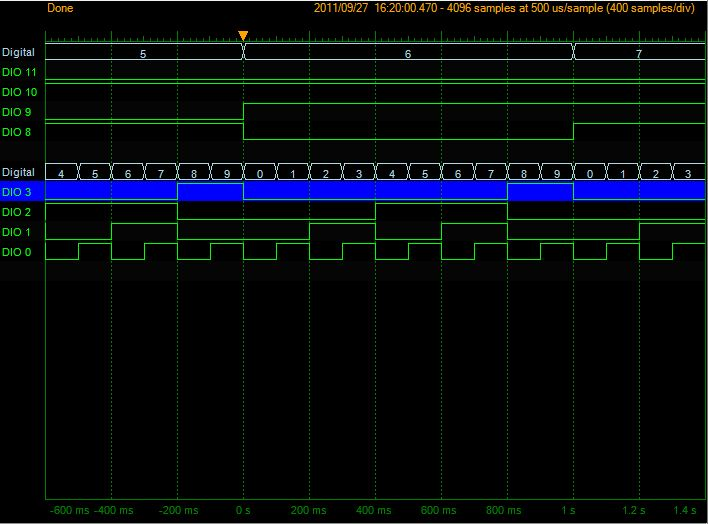
\includegraphics[width=300pt,keepaspectratio]{Figure1}
\caption{\small{Logic output of the two digits. DIO11-DIO8 correspond to the 
first digit,
and DIO3-0 correspond to the second digit. This demonstrates that the clock
increments in the right time, with the second digit incrementing every 0.1 seconds. }}
\end{figure}

\newpage\item \emph{Clock Count Output}
\\The clock count output was also tested using by using the digital local
analyser to ``watch'' the LED's. Figure 1 above and Figure 2 below both show
the count incrementing correctly. 
\begin{figure}[h!]
\centering
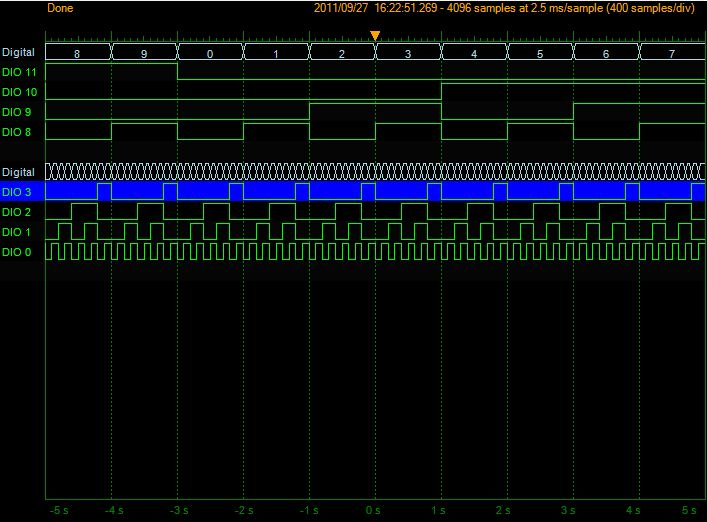
\includegraphics[width=300pt,keepaspectratio]{Figure2}
\caption{\small{Logic output of the two digits. DIO11-DIO8 correspond to the 
first digit,
and DIO3-0 correspond to the second digit. This demonstrates that that the count
does indeed reset after it reaches the maximum value.  }}
\end{figure}
\end{enumerate}

\newpage\emph{\textbf{Conclusion}}
\\The stop watch used three components: The Button Interface, the Timer Functionality,
and the Count Output. The button interface used a keypad and interupt routine. The
Timer Functionality used the internal clock to trigger an interupt to increment
the count. The count output was in BCD, with the first digit going to the first half
of a port and the second digit going to the second half of a port. The 
debugger and the digital logic analyzer tool were used to test the stop-watch. Based
on the clock count output, it seems that the stop-watch worked as it was meant 
to. 

\begin{thebibliography}{9}
\bibitem{Nelson}\emph{ELEC 3040 \& 3050 Laboratory Manual}\newline
\url{http://www.eng.auburn.edu/~nelsovp/courses/elec3040_3050}
\end{thebibliography}
\label{end}\end{document}
